\documentclass[12pt,oneside]{article}
\usepackage[utf8]{inputenc}
\usepackage[american]{babel}
\usepackage{bookmark}
\usepackage{microtype}
\usepackage[style=authoryear,sorting=nyt,backend=biber,
  hyperref=true,abbreviate=true,
  maxcitenames=1,maxbibnames=1]{biblatex}
  \renewbibmacro{in:}{}
  \addbibresource{../main.bib}
\usepackage{xcolor}
\usepackage{graphicx}
\pagecolor{green!3}
\usepackage{hyperref}
  \hypersetup{colorlinks=true,allcolors=blue!40!black}
\setlength{\topskip}{6pt}
\setlength{\parskip}{6pt} % before par

\DeclareCiteCommand{\citea}
  {\boolfalse{citetracker}\boolfalse{pagetracker}\usebibmacro{prenote}}
  {\href{\thefield{url}}{\printnames{labelname}}}
  {\multicitedelim}
  {\usebibmacro{postnote}}

\def\zoldversion{0.2.4}

\title{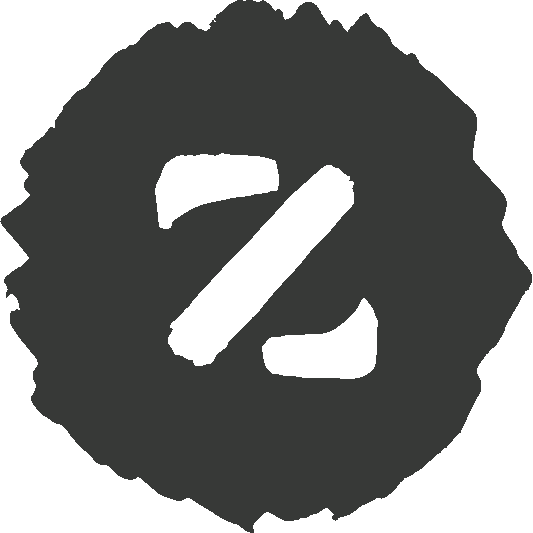
\includegraphics[scale=0.3]{../images/logo.pdf}\\Zold: A New Cryptocurrency\\\colorbox{green!30}{Green Paper}}
\author{Yegor Bugayenko\\
  \texttt{yegor256@gmail.com}\\
  \href{https://www.zold.io}{www.zold.io}\\[1em]
  \href{https://github.com/zold-io/papers/releases/tag/\zoldversion}{\texttt{\zoldversion}}}

\begin{document}
\raggedbottom

\maketitle

In the last few years digital currencies have successfully demonstrated
their ability to become an alternative financial instrument in many
different markets. Most of the technologies available at the moment are
based on the principles of \href{https://en.wikipedia.org/wiki/Blockchain}{Blockchain} architecture, including
dominating currencies like \href{https://bitcoin.org/}{Bitcoin} and
\href{https://ethereum.org/}{Etherium}. Despite its
popularity, Blockchain is not the best possible solution for all scenarios.
One such example is for fast micro-payments.
\href{https://www.zold.io}{Zold} is an experimental alternative
that enables distributed transactions between
anonymous users, making micro-payments financially feasible and fast.
It borrows the ``\href{https://en.wikipedia.org/wiki/Proof-of-work_system}{proof of work}'' principle from Bitcoin,
and suggests a different architecture for digital wallet maintenance,
explained in details in the \href{https://papers.zold.io}{White Paper}.

\pagebreak

\section*{The Market}

Since its release in 2009, Bitcoin from
``a libertarian fairy tale'' and ``a simple Silicon Valley exercise in hype''
turned into ``a catalyst to reshape the financial system in ways that are more
powerful for individuals and businesses alike,'' according to \citea{andreessen2014}.
Even though \citea{cheah2015} argues that
``the fundamental value of Bitcoin is zero,''
it seems that ``the question is not whether Bitcoin has value; it already does,''
according to \citea{van2014}.
``The question is whether the efficiencies of a cybercurrency
like Bitcoin can be merged with the certainties of an honest central bank.''

The core component of Bitcoin is Blockchain technology, which
``ensures the elimination of the double-spend problem, with the help
of public-key cryptography'' and ``coins are transferred by the
digital signature of a hash,''
explains \citea{pilkington2016}.
Very soon after Bitcoin was created, similar products were introduced,
which were also based on the principles of Blockchain, such as
Etherium by \citea{buterin2013}.

Even though Blockchain is a sound solution to the double-spending
problem, there could be other solutions,
including different ``proof-of-X'' alternatives.
For example, \citea{everaere2010} gave
a summary of them and introduced their own,
\citea{boyen2016} described
``a truly distributed ledger system based on a lean graph of cross-verifying transactions,''
recently \href{https://www.iota.org/}{IOTA}, a ``tangle-based cryptocurrency,'' was launched by
\citea{popov2017},
\citea{hashgraph} claims to be ``the world's first mass-adopted public distributed ledger'',
and so on.

\pagebreak

\section*{The Problems}

Zold is also a decentralized digital currency that maintains its ledgers
through an unpredictable amount of anonymous and untrustable server nodes, trying to guarantee
data consistency. The architecture of Zold is not Blockchain-based.
The development of Zold was motivated by the desire to overcome
two obvious disadvantages present in the majority of all existing cryptocyrrencies:

The first problem is that transaction processing is rather slow.
\href{https://goo.gl/sWiAWc}{Current rates} for Bitcoin processing speed is 7 transactions per second (tps)
while Paypal handles an average of 115 tps and the VISA
network has a peak capacity of 47,000 tps.
\citea{karame2012} says that
``Bitcoin requires tens of minutes to verify a transaction
and is therefore inappropriate for fast payments.''
It is inevitable, since
``processing speed is at odds with the security aspects of the underlying
proof-of-work based consensus mechanism'' according
to \citea{kiayias2015}.
Ethereum, according to \citea{fekkes2018}, can process
``two times more transactions per second than Bitcoin is able to do,''
but this still is rather slow.

The second problem, as noted by \citea{popov2017},
is that ``it is not easy to get rid
of fees in the blockchain infrastructure since they serve
as an incentive for the creators of blocks.''
\citea{moser2015} says that ``Bitcoin users are encouraged to
pay fees to miners, up to 10 cents (of USD) per transaction, irrespective of the
amount paid'' which especially hurts when transaction amounts are smaller than a dollar.
Moreover, according to \citea{kaskaloglu2014},
``an increase in transaction fees of Bitcoin is inevitable.''

Thus, the speed is low and the processing fees are high.
Zold was created as an attempt to resolve these two problems.

\pagebreak

\section*{The Features}

Unlike all other crypto currencies, there is no central ledger in Zold.
Each wallet has its own personal ledger.
All transactions in each ledger are confirmed by
\href{https://en.wikipedia.org/wiki/RSA_(cryptosystem)}{RSA} signatures of their owners.

Similar to many other digital currencies---including
Bitcoin, Etherium, \href{https://getmonero.org/}{Monero},
\href{https://plancoin.co/}{Plancoin}, \href{https://dero.io/}{Dero},
and many others---Zold nodes find consensus by using the CPU power invested
by each of them to perform certain expensive and meaningless calculations
that result in finding hash suffixes, also known as ``proof-of-work,''
initially introduced by \citea{back1997} in \citeyear{back1997}.

Zold is a pre-mined digital asset, similar to
\href{https://ripple.com/}{Ripple},
\href{https://www.cardano.org/en/home/}{Cardano},
\href{https://www.stellar.org/}{Stellar},
\href{https://neo.org/}{NEO}, and many others.
One currency unit is called ZLD.
Therefore, the technical capacity of the currency is 2,15 billion ZLD.
To compare, the total supply of some crypto currencies is:
Bitcoin: 21m BTC, Ripple: 100b XRP,
\href{https://litecoin.org/}{Litecoin}: 84m LTC,
\href{https://www.dash.org/}{Dash}: 19m DASH.

Zold has two obvious advantages comparing to many other
similar solutions: it is fast and cheap. First, the speed of transaction processing
literally has no limits, because all payments are made locally, on users'
machines. Second, the cost of transaction processing
is lower than most other payment systems can offer. To process
a thousand transactions a user has to pay \$500 in Bitcoin and \$300 in Ethereum,
while in Zold it is as little as \$4.

\end{document}
